%\sectskip
\vspace{-5pt}
\section{Certifying the {\mCTOS} Kernel}
\label{sec:base}
%\asectskip

\ignore{
\begin{figure}
\begin{minipage}{.22\textwidth}
\lstinputlisting [language = C] {source_code/lock_producer.c}
\end{minipage}\hfill
\begin{minipage}{.22\textwidth}
\lstinputlisting [language = C] {source_code/lock_consumer.c}
\end{minipage}
\ifTR{}{\vspace*{-5pt}}
\caption{Lock-based producer-consumer implementation}
\label{fig:exp:lock}
\end{figure}
}


\begin{comment}
\begin{figure*}
\begin{center}
\begin{scriptsize}
\begin{tabular}{ |l|l||l|p{4.5cm}| }
  \hline
  \multicolumn{2}{|c||}{\textbf{Memory Management}} 
  & \multicolumn{2}{|c|}{\textbf{Thread and Process Management}} \\
  \hline
  \hline    
  \multicolumn{2}{|l||}{\textbf{abstract state}} 
  & \multicolumn{2}{|l|}{\textbf{abstract state}}\\
  \hline
  \verb"AT" & physical page allocation table
  & \verb"kctxp" & kernel context (\verb"kctx") pool\\
  \hline 
  \verb"PFInfo" & save the address and \verb"PC" that page fault occurs
  & \verb"Ltdqp" & low abstract thread queue pool\\
  \hline
  \verb"ptp" & page table (\verb"pt") pool 
  
  & \verb"Htdqp"& high abstract thread queue (\verb"Htdq") pool\\ 
  \hline
   \verb"ipt"& whether \verb"pt"'s invariant  should hold or not
  
  & \verb"uctxp" & user context pool\\
  \hline
\verb"PT" & index of the current \verb"pt"
  & \verb"chanp" & channel pool\\
  \hline
  \verb"pbit" & bit map for free \verb"pt" indexes
  & \verb"Htcbp"& high abstract TCB pool \\
  \hline
  \multicolumn{2}{|l||}{\textbf{primitive}} 
  & \multicolumn{2}{|l|}{\textbf{primitive}}\\
  \hline	
  \verb"setcr3" & set the starting address of the \verb"pt"
  & \verb"kctx_new" & allocate the first free \verb"pt" and \verb"kctx"\\
  \hline
  \verb"meminit" & initialize the allocation table
  & \verb"Henqueue" & append a thread to the \verb"Htdq"\\
  \hline
  \verb"palloc" & allocate a page 
  & \verb"thread_kill" & kill and free a thread\\
  \hline
  \verb"pt_insrt" & insert a page map into a given \verb"pt" 
  & \verb"thread_sleep" & sleep, schedule to the 1st ready thread\\
  \hline
  \verb"pt_resv" & allocate a page for a given linear addr 
  & \verb"kctx_switch" & switch \verb"kctx" between threads\\
  \hline 
  \verb"PTInit" & init kernel's \verb"pt" and enable paging 
  & \multirow{2}{*}{\texttt{resv\_chan}} & 
  receive msg from the channel, wake\\
  \cline{1-2}
  \verb"pt_new" & allocate the first free \verb"pt" & & up the first sleeping thread
    \\	  
  \hline
  \hline
  \multicolumn{2}{|c||}{\textbf{Virtualization}}
  &\multicolumn{2}{|c|}{\textbf{Trap Handler}} \\
  \hline
  \hline    
  \multicolumn{2}{|l||}{\textbf{abstract state}} 
  & \multicolumn{2}{|l|}{\textbf{primitive}} \\
  \hline
  \verb"npt" & nested page table for guest
  & \verb"trap_arg" & get arguments of system calls\\
  \hline
  \verb"hctx"& host context
  & \verb"hpagefault" & page fault handler\\ 
  \hline
  \verb"vmcb" & virtual machine (\verb"VM") control control block
  & \verb"sys_yield" & system calls for yielding\\
  \hline
  \verb"xvmst" & registers not saved in \verb"vmcb" 
  & \verb"sys_wait_chan" & system calls to sleep on a channel\\
  \hline
  \multicolumn{2}{|l||}{\textbf{primitive}} 
  & \verb"sys_run_vm" & system calls to run \verb"VM"\\
  \hline	
  \verb"npt_insrt" & insert into the nested page table
  & \verb"sys_proc_create" & system calls to create a process\\
  \hline
  \verb"switch2guest" &  switch to guest mode 
  & \verb"sys_getexitinfo" 
  & get the information about \verb"VM" exit\\
  \hline
  \verb"set_vmcb" & set value in virtual machine control block
  & \verb"sys_injectevent" & inject interrupt and exception to \verb"VM"\\
  \hline 
  \verb"run_vm" & save host context, restore \verb"vmcb", start \verb"VM" 
  & \verb"kernel_init" & initialization function of the kernel\\  
  \hline  

\end{tabular}
\end{scriptsize}
\caption{Key abstract states and primitives for \mCTOSbase{} and \mCTOShyper{}}
\label{table:layers}
\end{center}
%\vspace*{-14pt}
\end{figure*}
\end{comment}

\begin{comment}
\begin{figure}
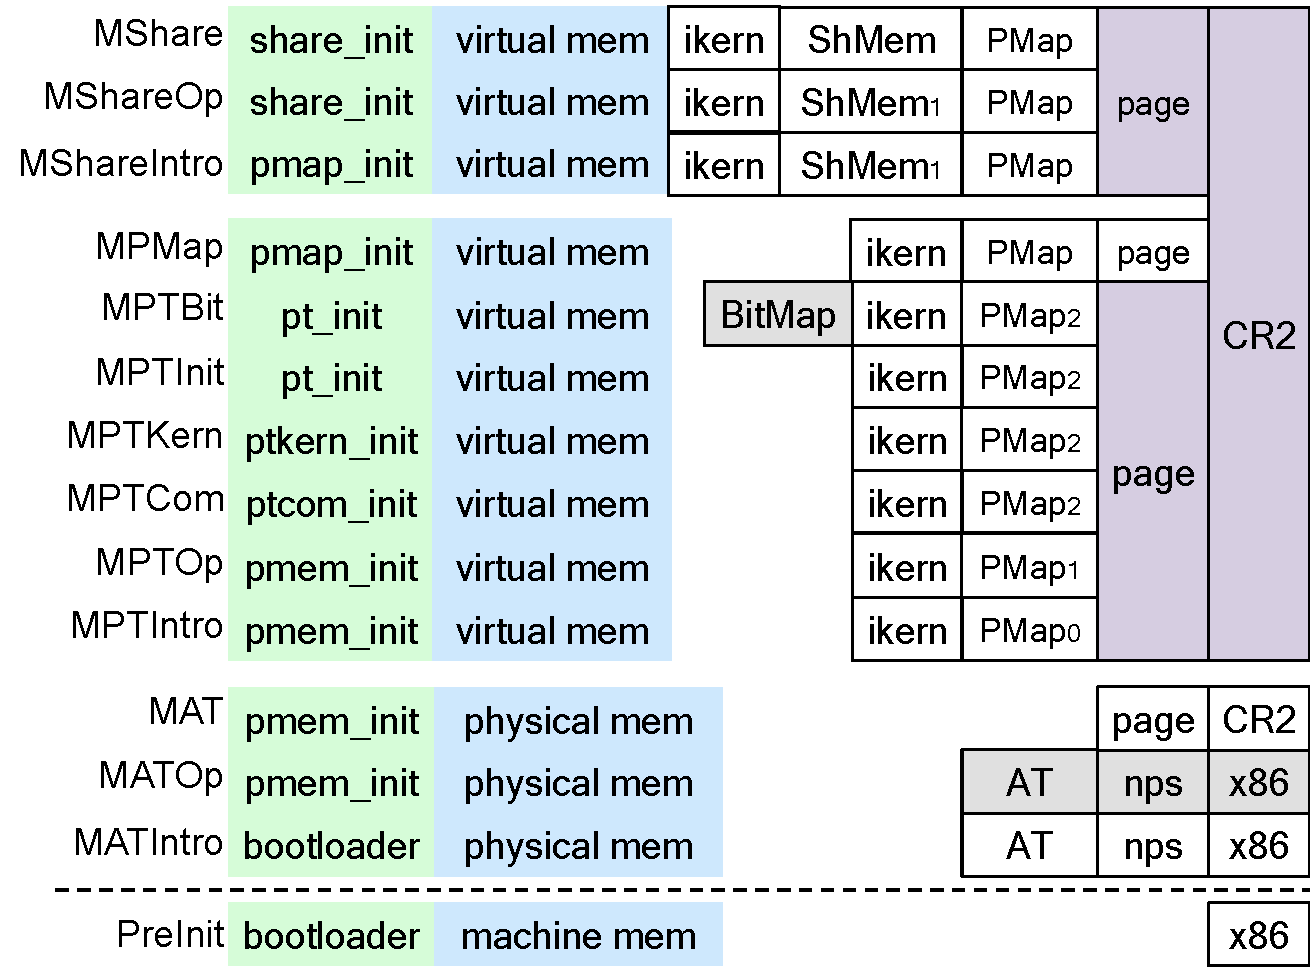
\includegraphics[scale=0.38]{figs/memory_management_layer}	
\caption{Layers of PreInit and memory management}
\label{fig:base:mm:layers}
\vspace*{-14pt}
\end{figure}

\begin{figure}
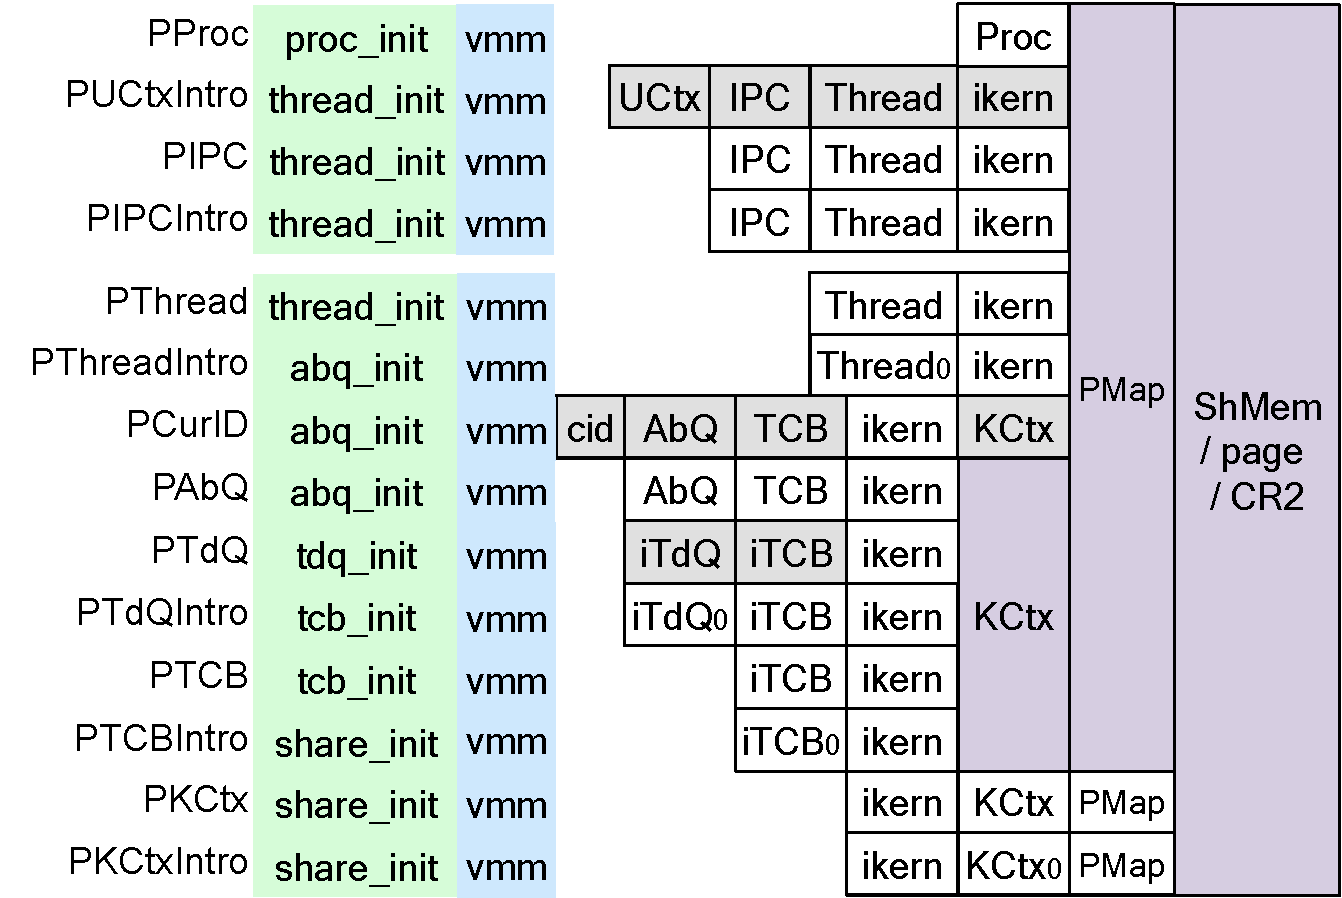
\includegraphics[scale=0.37]{figs/process_management_layer}	
\caption{Layers of process management}
\label{fig:base:pm:layers}
\vspace*{-14pt}
\end{figure}

\begin{figure}
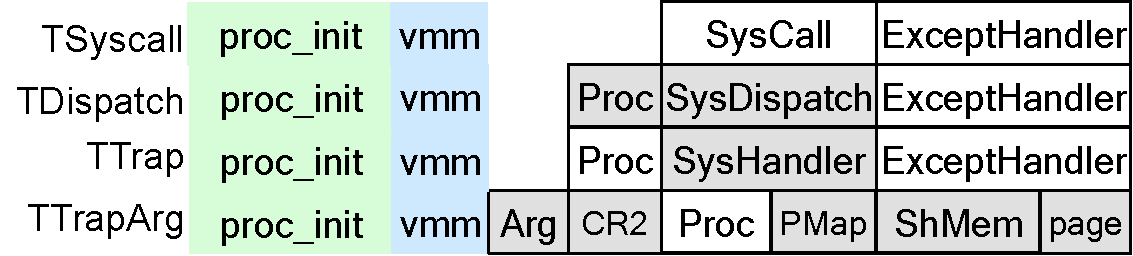
\includegraphics[scale=0.37]{figs/trap_management_layer}	
\caption{Layers of trap management}
\label{fig:base:tm:layers}
\vspace*{-14pt}
\end{figure}
\end{comment}

\ignore{
\begin{figure}
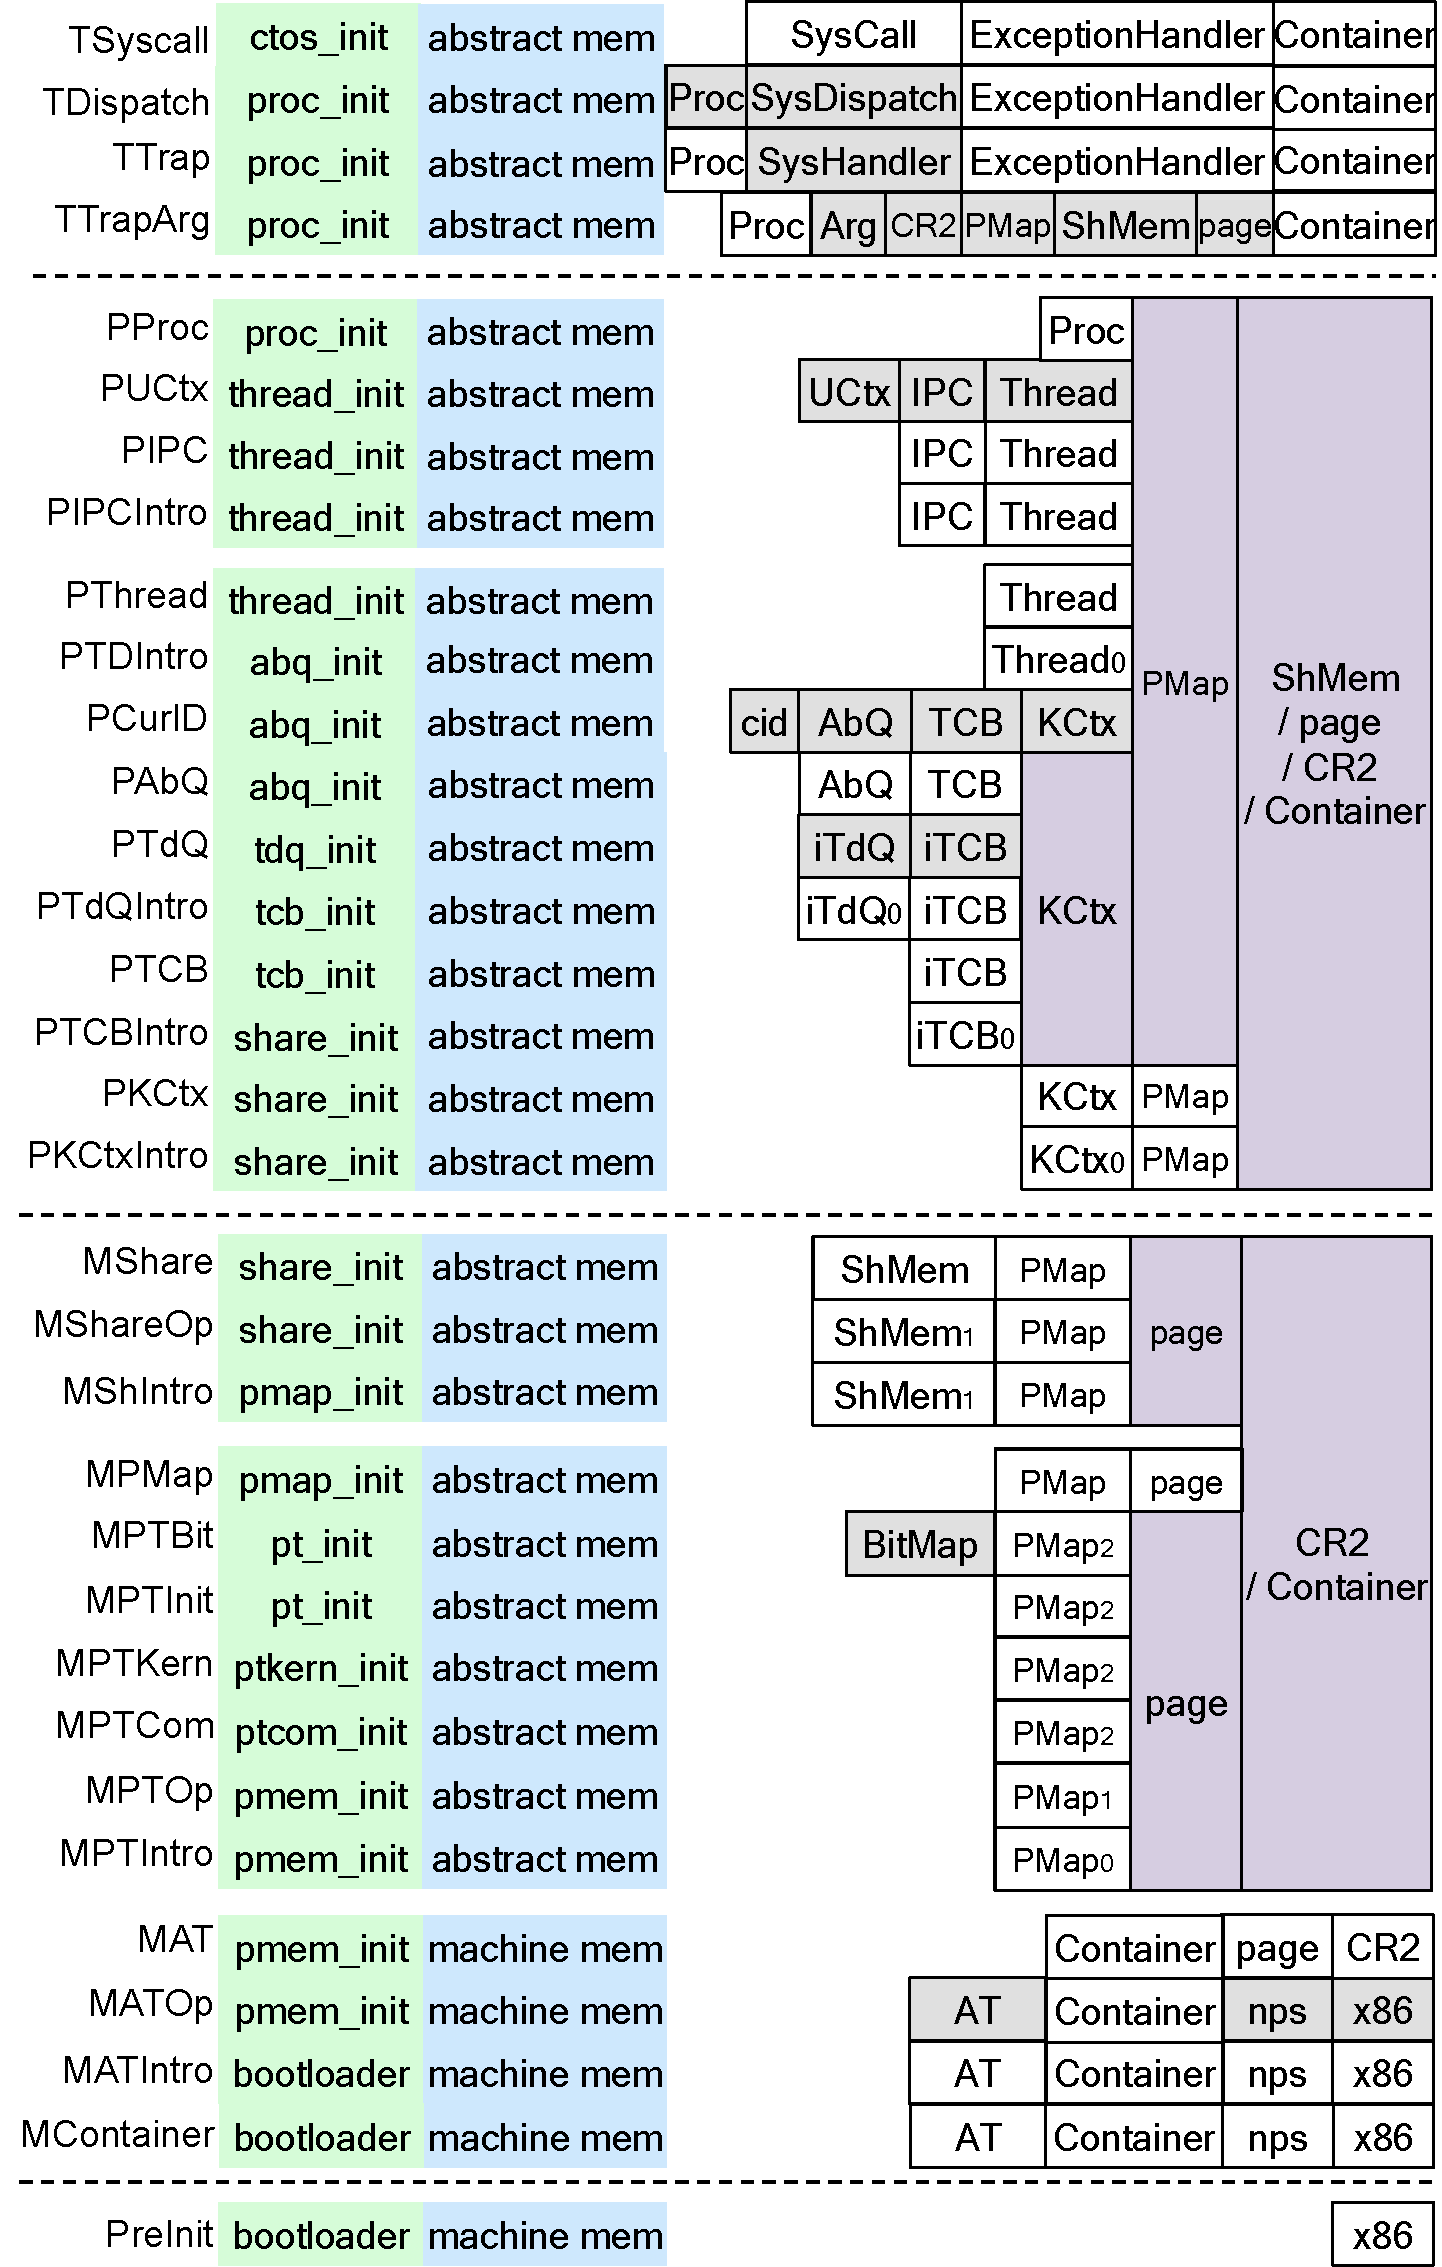
\includegraphics[scale=0.34]{figs/mctos_layer}	
\caption{Layers of \mCTOSbase{}}
\label{fig:base:ctos:layers}
\vspace*{-14pt}
\end{figure}
}

In this section, we present the main components of the certified {\mCTOS} kernel. 
The pre-initialization module is the bottom layer that connects to the
 \emph{CPU-local machine model} $\mach{loc}$, instantiated with a 
 particular \emph{active CPU} (\cf Sec.~\ref{subsec:spec:seq}).
The trap handler contains the top layer that provides system call interfaces
and serves as a specification of the whole kernel,
instantiated with a particular active thread
running on that active CPU.
Our main theorem states that any global properties proved at the topmost
abstraction layer can be transferred down to the lowest hardware machine.
In this section, we explain selected components
in more details.

\ignore{
\paragraph{Pre-initialization module}
\label{sec:base:preinit}
only contains the bottommost layer
\code{PreInit}. It axiomatizes the x86 hardware behaviors of a particular active CPU.
These behaviors include page table walk upon memory load when paging is turned on, 
saving and restoring the trap frame in the case of interrupts and exceptions (\eg, page fault), 
and the data exchange between devices and memory.
\ignore{The abstract state of the \code{PreInit} layer consists of control registers, FLAGS registers,
registers of devices, an E820 memory map \code{MM} (set up by the bootloader),
and a CPU-mode flag (either kernel or user mode).
\ignore{Its primitives consist of
getter-setter functions for control registers and \code{MM},
and a function models the transition between user and kernel mode.}
}

As shown in Fig.~\ref{fig:spec:memmodel}(a),
the hardware memory management unit (MMU) is modeled 
in a way that mirrors the paging hardware.
When paging is enabled (as indicated by \code{CR0}),
memory accesses made by both the kernel and the user programs
are translated using the page map pointed to by \code{CR3}.
When a page fault occurs,
the fault information is stored in \code{CR2},
the CPU mode is switched from user mode to kernel mode,
and the page fault handler is triggered.
}
\ignore{
Some privileged
memory regions (\eg, allocation table) and 
instructions (\eg, modifying control registers)
are only available in kernel mode.}
\ignore{
\code{CR0} selects the memory protection mode,
\code{CR2} stores the Page Fault Linear Address (PFLA)
as well as the address of the instruction that caused the page fault, and
\code{CR3} stores the starting point of the page map.
}
\ignore{
The switch function models the change of the \code{ikern} flag
and the remaining tasks involved with trap handling,
such as saving and restoring user and kernel contexts,
and dispatch over the trap type,
are verified at the assembly level.
}


\ignore{
{\color{red}Jan: Do we need the following paragraph?}
The initialization primitive at this bottom-most layer is the bootloader,
which initializes \code{MM} and necessary drivers
(tsc, disk, console, timer, keyboard, serial, {\it etc.}),
loads the kernel into the memory,
and sets the initialization flag to be \code{true}.
}

\paragraph{Lock module}
\label{sec:base:lock}
of the {\mCTOS} kernel provides fine-grained lock objects
as the base of synchronization mechanisms.

\begin{figure}
\lstinputlisting [language = C, multicols=2] {source_code/ticket_lock.c}
\vspace{-5pt}
\caption{Pseudocode of ticket lock implementation.}
\label{fig:exp:ticket_lock}
\vspace{-10pt}
\end{figure}

\textbf{Ticket Lock}
depends on an \emph{atomic ticket object}, which consists of two 
fields: \code{ticket} and \code{now}.
Figure~\ref{fig:exp:ticket_lock} shows one implementation of a
ticket lock. The atomic increment to the ticket is achieved
through the atomic \texttt{fetch-and-increment} (FAI) operation (implemented using
the \texttt{xaddl} instruction with the \texttt{lock} prefix in x86).
As described in Sec.~\ref{subsec:spec:seq}, 
the \emph{{\intptext}s} at this abstraction level have been shuffled and merged so that there is exactly one {\intptext}
in front of each atomic operation. 
Thus, the lock implementations generate a list of events;
\ignore{The atomic operations generate ticket-object events;}
for example, when CPU $t$ attempts to acquire the lock $i$, it continuously generates 
the event ``$\event{t.get\_now\ i}$" (line~9)
until the latest \code{now} is increased
to the ticket value returned by the event ``$\event{t.inc\_ticket\ i}$" 
(line~8), and then followed by the event ``$\event{t.pull\ i}$" (line~10):\vspace{-5pt}
\[
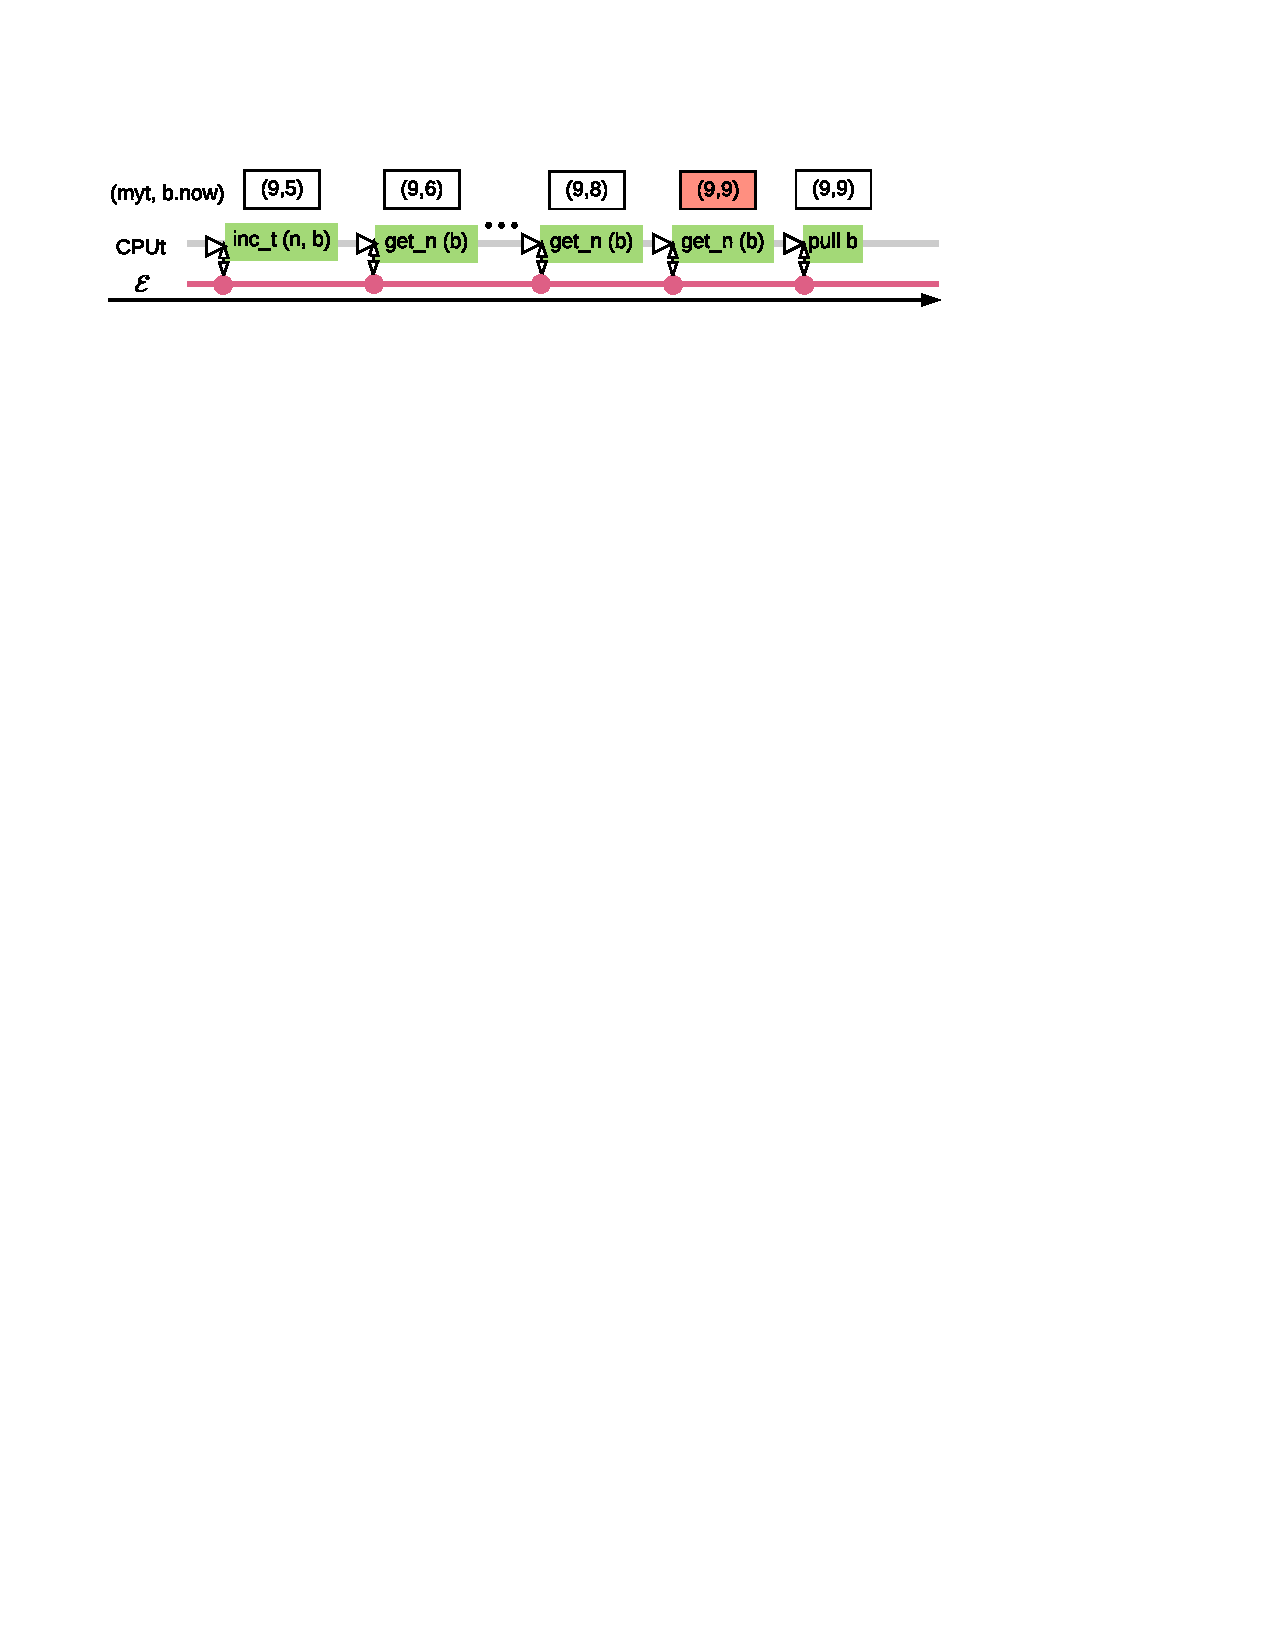
\includegraphics[scale=.6]{figs/ticket_log}
\vspace{-5pt}
\]
\ignore{
The event list is as below:
$$[\intp,\event{t.inc\_ticket\ i},\intp,\event{t.get\_now\ i},\cdots,\intp,\event{t.get\_now\ i}]$$
}

Certifying the atomic ticket lock object consists of two main proof obligations:
(1) the lock guarantees \emph{mutual exclusion}, and (2) the lock  
is \emph{starvation-free}.

\emph{Mutual exclusion}
is straightforward for a ticket lock.
At any time, only the thread whose ticket is equal to
the current serving ticket (\ie, \code{now})
can hold the lock. 
Furthermore, each thread's ticket is unique
as the $\texttt{fetch-and-increment}$ operation is atomic
(line 8). 
Thanks to this \emph{mutual exclusion} property,
it is safe to \emph{pull} the shared memory associated with
the lock $i$ to the local copy
at line 10.
Before releasing the lock, the local copy is \emph{pushed}
back to the shared memory at line 13.

\emph{Starvation-freedom} can be proved
by showing that lock acquire eventually succeeds.
To prove this, we impose a set of invariants on the environment
context at this layer.

\vspace{-3pt}
\begin{invariant}[Invariants for ticket lock]
\label{inv:lock}
An environment context that holds the lock $i$,
(1) never acquires lock $i$ again before releasing it;
and (2) always releases lock $i$ within $k$ steps
(for some $k$).
\end{invariant}
Furthermore, we assume the hardware scheduler $\hardoracle$ is \emph{fair},
meaning that between any two consecutive events from the same thread,
there are less than $m$ events generated by other threads (for some $m$).

\vspace{-3pt}
\begin{lemma}[Starvation-freedom of ticket lock]
\label{lemma:lock}
Acquiring ticket-lock in the {\mCTOS} kernel eventually succeeds.
\ignore{\proof 
Let $n$ be the maximum number of the threads in the system.
Then (1) there are at most $n$ threads waiting before the current one;
(2) the thread holding the lock releases the lock within $k$ steps,
which generates at most $k$ events;
(3) environment context generates less than $m$ events between each step of the lock holder;
and (4) every \code{get\_now} generates one event.
Hence there are at most
$n\times m\times k$ loop iterations at line 10 in Fig.~\ref{fig:exp:ticket_lock},
and so acquiring lock always succeeds.
\qed}
\end{lemma}
Once we prove starvation freedom,
we abstract the lock implementation into atomic specifications in
the higher layers such that acquiring a lock only generates a single
event ``$\event{t.acq\_lock\ i}"$. To compose the specification with
the environment context, we prove that Invariant~\ref{inv:lock}
holds on the current CPU at overlay.

\ignore{
\begin{figure}
\lstinputlisting [language = C, multicols=2] {source_code/mcs_lock.c}
\caption{MCS Lock Implementation}
\label{fig:exp:mcs_lock}
\end{figure}
}

\textbf{MCS Lock} is known to have better scalability than ticket lock
on large numbers of CPUs.
In the {\mCTOS} kernel, we have also implemented a version of MCS 
locks~\cite{Mellor-Crummey:mcs-locks}.
The starvation-freedom proof is similar to that of the ticket lock. 
The difference is that the MCS lock release operation waits in a loop until the next waiting thread (if it exists)
has added itself to a linked list, so we need similar proofs for both acquire and release.

\vspace{-3pt}
\paragraph{Device drivers}
\label{sec:base:device}
Chen {\it et al} \cite{chen16} present a framework to allow interrupts
inside the kernel
with device drivers. \ignore{The core idea is to treat device drivers of
each device as if they were running on a ``logical'' CPU dedicated to that device,
and build a framework that systematically enforces the isolation among different
``devices'' and the rest of the kernel.} The work has been successfully ported
into our setting relatively easily thanks to the fact that their event-based
 model is consistent with our interleaving machine model.


\ignore{\subsection{Memory management}
\label{sec:base:memm}

The memory management of {\mCTOS} consists of  the
\emph{physical memory management} (4 layers), 
\emph{virtual memory management} (7 layers), and
\emph{shared memory management} (3 layers).
}

\ignore{
\begin{figure}
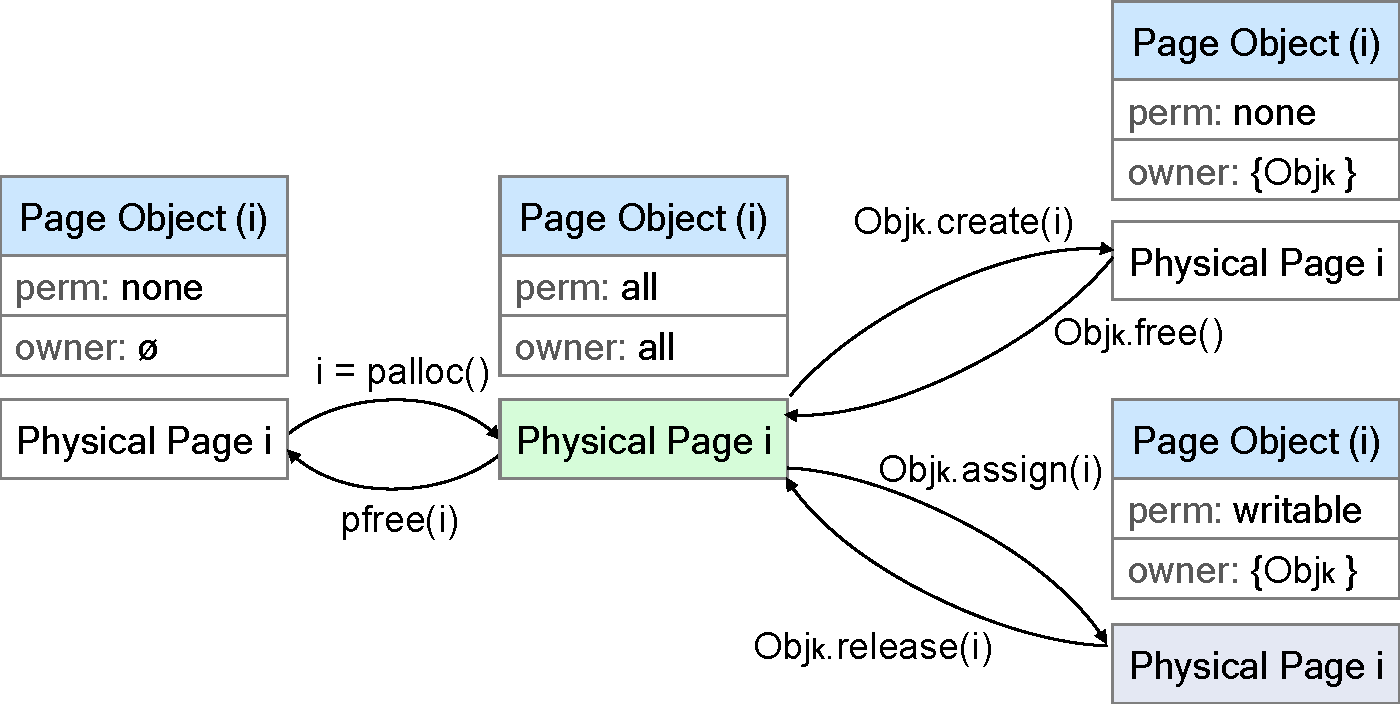
\includegraphics[scale=0.35]{figs/dynamic}	
\caption{The state transition of page object}
\label{fig:base:dynamic}
\vspace*{-14pt}
\end{figure}
}

\vspace{-3pt}
\paragraph{Physical memory management}
\label{sec:base:memm}
maintains the physical pages and provides a \emph{dynamic page allocator}
\texttt{palloc} (\cf Fig.~\ref{fig:exp:palloc}).
As the page allocation table $\texttt{AT}$ is shared among different CPUs, 
we associate it with a lock $\texttt{lock\_AT}$.
The dynamic page allocator is then refined into an atomic object where
the \texttt{palloc} implementation is proved to satisfy an atomic interface,
with the proof that
lock utilization for $\texttt{lock\_AT}$ satisfies Invariant~\ref{inv:lock}.
Once the dynamic page allocator is introduced as
 an atomic object, the lock acquire and lock release 
for $\texttt{lock\_AT}$
are \emph{not allowed to be invoked} at higher layers. 
Thus, in this layered approach, it is not possible
that a thread holding a lock defined in a lower layer tries to acquire another lock
introduced in a higher layer, \ie, the order that a thread acquires different
locks is guided by the order that the locks are introduced in the layers.
This implicit order of lock acquisitions prevents \emph{deadlocks} in the
{\mCTOS} kernel.

\begin{figure}
\lstinputlisting [language = C, multicols=2] {source_code/palloc.c}
\vspace{-5pt}
\caption{Pseudocode of \texttt{palloc}}
\label{fig:exp:palloc}
\vspace{-10pt}
\end{figure}



Another function of the physical memory management is to dynamically
track and bound the memory usage of each thread. A \emph{container}
object is used to record information for each thread (array \code{cn}
in Fig.~\ref{fig:exp:palloc}); one piece of information tracked is the
thread's \emph{quota}. Inspired by the notions of containers and
quotas in HiStar~\cite{zeldovich06}, a thread
in {\mCTOS} is spawned with some quota specifying the maximum number
of pages that the thread will ever be allowed to allocate. As can be
seen in Fig.~\ref{fig:exp:palloc}, \code{palloc} returns an error
code if the requesting thread has no remaining quota (lines~4 and~5), 
and the quota is decremented when a page is successfully allocated (line~17).
Quota enforcement allows the kernel to prevent a denial-of-service attack,
where one thread repeatedly allocates pages and uses up all available
memory (thus denying other threads from allocating pages). From a security
standpoint, it also prevents the undesirable information channel between 
different threads that occurs due to such an attack.


\begin{figure*}[th]
$$
\begin{array}{c|c}
\begin{array}{cc}
(a) &\
      \begin{array}{c}
			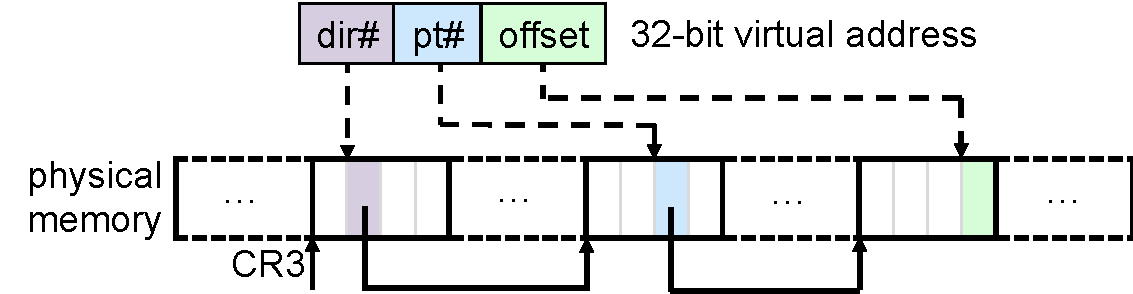
\includegraphics[scale=.33]{figs/mem_model_1} 
		\end{array}
\end{array}
& 
\begin{array}{cc}
(b) & 
\begin{array}{c}
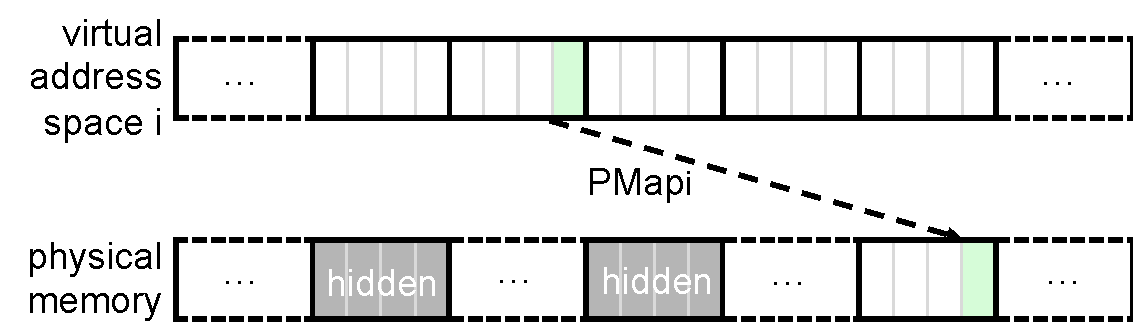
\includegraphics[scale=.35]{figs/mem_model_2}
\end{array}
\end{array}
\vspace*{-14pt}
\end{array}
$$
\caption{(a) Hardware MMU using two-level page map; (b) Virtual address space $i$ set up by page map $i$.}
\label{fig:spec:memmodel}
\vspace*{-10pt}
\end{figure*}

\vspace{-3pt}
\paragraph{Virtual memory management}
provides consecutive virtual address spaces on top of physical memory management.
Because much of the code assumes that 
the memory management sets up the virtual address space properly,
initialization has been a sticking point.
We proved not only that the primitives of virtual memory management
manipulate the page maps correctly,
but also that the \emph{initialization procedure} sets up the two-level page maps properly
in terms of the hardware address translation.


\begin{invariant}
\label{inv:virtual}
1) paging is enabled only after the initialization of virtual memory management;
2) the memory regions that store kernel-specific data must have the kernel-only 
permission in all page maps;
3) the page map used by the kernel is an identity map
4) the non-shared parts of user processes' memory are isolated (see 
Sec.~\ref{security}).
\end{invariant}


By Inv.~\ref{inv:virtual}, we show that it is safe to
run both the kernel and user programs in the virtual 
address space when paging is enabled.
In this way, memory accesses at higher layers
operate on the basis of
the high-level, abstract descriptions of address spaces
rather than concrete page directories and page tables stored in the memory
itself.


\vspace{-3pt}
\paragraph{Shared memory management} provides a protocol to share physical
pages among different user processes. 
It provides an infrastructure to map a physical page into multiple
processes' page maps (\ie, processes' address spaces).
We prove that the shared page can only be freed after 
all processes release their ownership of that page.

\ignore{
Its verification makes use
of the ownership relation. 
For example, a user process $k_1$ can share its private physical page $i$
to another user process $k_2$ through the shared memory protocol,
and the owner set of page object $i$ will become
$\{\text{process object }k_1, \text{process object }k_2\}$.
}


\ignore{\subsection{Process management}


Process management  introduces the
\emph{abstract queue library} (4 layers),
\emph{thread management} (6 layers),
\emph{condition variable} (3 layers),
and \emph{IPC} module (2 layers).}

\ignore{\begin{figure}
\lstinputlisting [language = C, multicols=1] {source_code/enqueue.v}
\vspace{-5pt}
\caption{Specifications of local queue operations.}
\label{fig:exp:queue}
\vspace{-10pt}
\end{figure}}


\vspace{-3pt}
\paragraph{Abstract queue library}
\label{sec:base:procm} abstracts the queues implemented as \emph{doubly-linked lists}
into \emph{abstract queue states} (\ie, Coq lists).
The local {\it enqueue} and {\it dequeue} operations
are specified over the abstract lists.
As usual, we associate each shared queue with a lock.
The atomic interfaces for shared queue operations are represented by
queue events $``\event{t.enQ\ i\ e}"$ and 
$``\event{t.deQ\ i}"$,
which can be replayed to construct the shared queue. 
For instance, starting from an empty initial queue,
the resulting queue constructed from
the log of the following interleaving
is $[2,5]$. \vspace{-5pt}
\ignore{and the last atomic dequeue operation returns 3.}
\ignore{ 
if the current local log of $i$'th shared queue is
$[\intp,\event{t_0.enQ\  i\ 2},\intp,\event{t_0.deQ\ i}]$,
and the event lists generated by the \emph{environment context} at two {\intptext}s are
$[\event{t_1.enQ\  i\ 3},\event{t_1.enQ\  i\ 4}]$ and
$[\event{t_1.enQ\  i\ 5}]$, respectively,
then the complete logical log for the shared queue $i$ is:}
\[
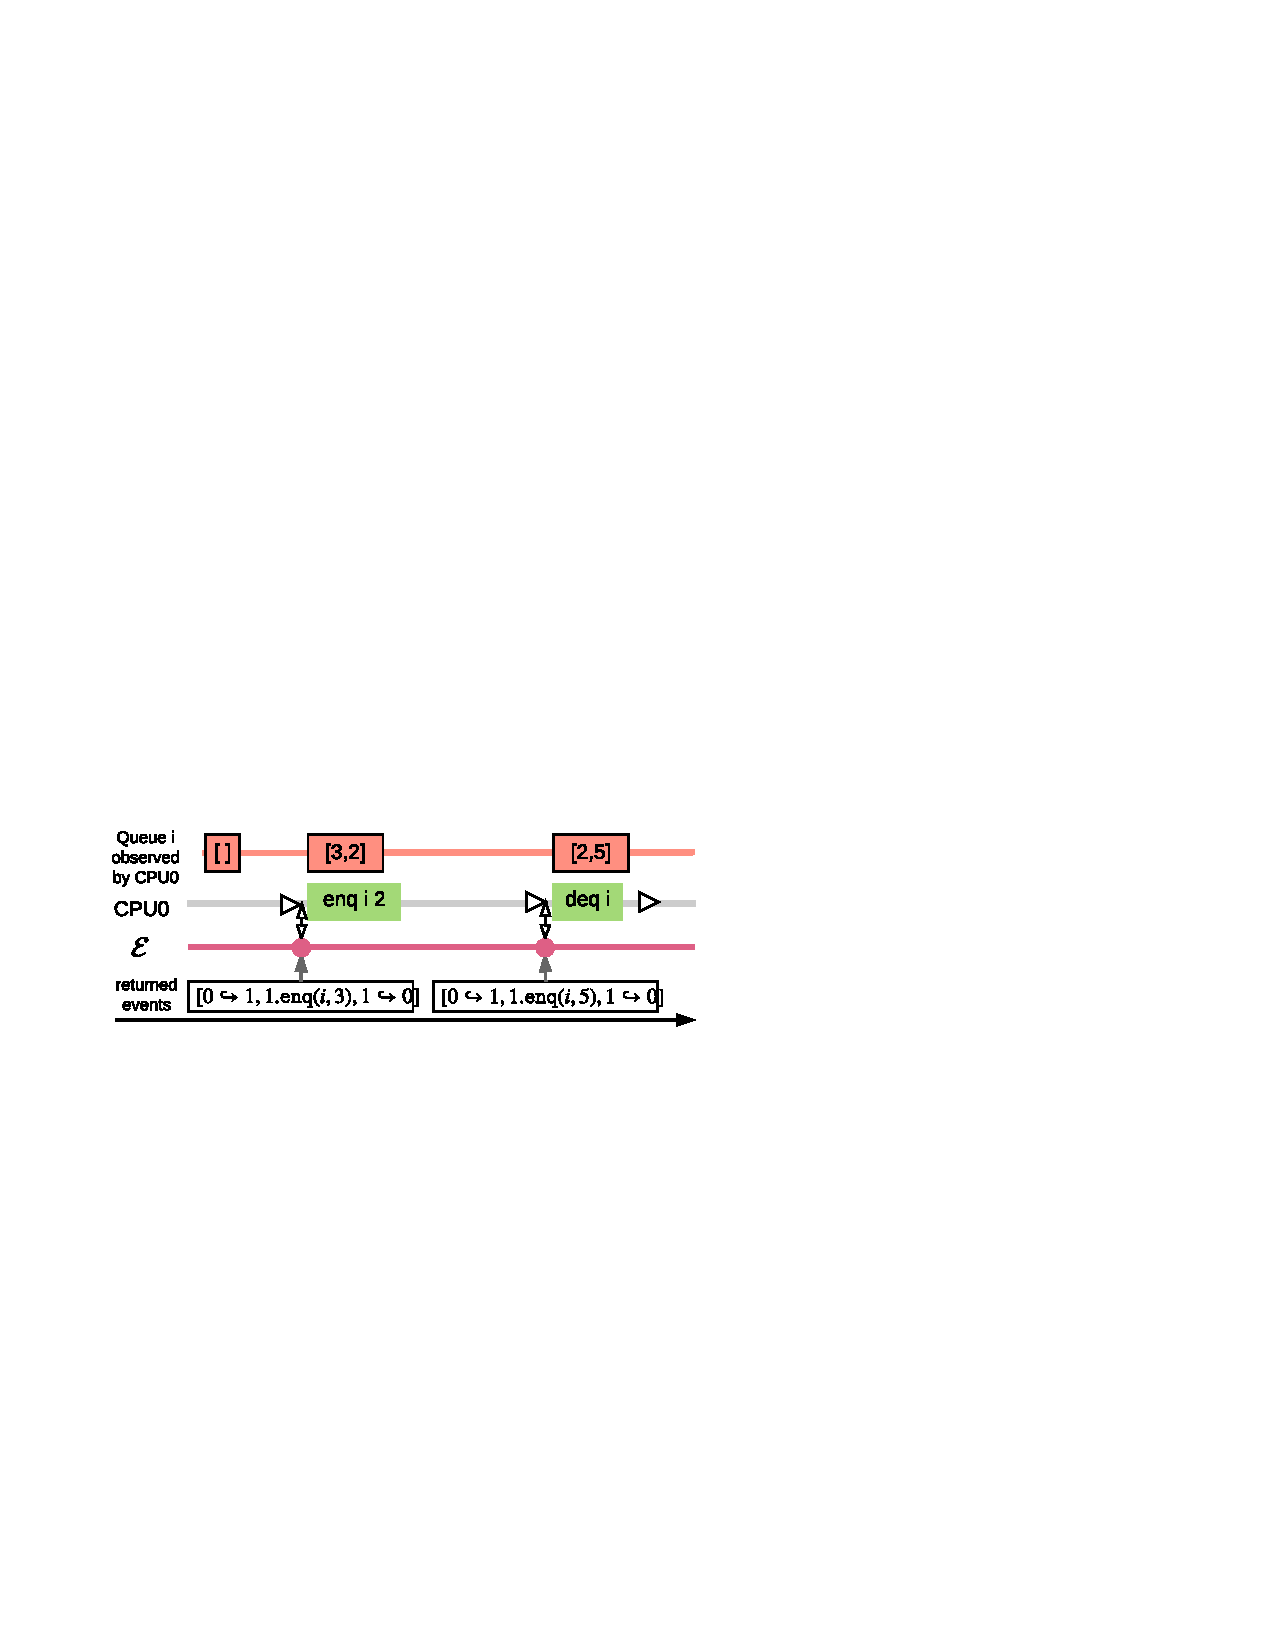
\includegraphics[scale=.65]{figs/queue_log}
\]
\ignore{
$$[\event{t_1.enQ\  i\ 3},\event{t_1.enQ\  i\ 4},\event{t_0.enQ\  i\ 2},\event{t_1.enQ\  i\ 5},\event{t_0.deQ\ i}]$$
}

\ignore{Thus, by replaying the log, the shared queue state is calculated as $[4,2,5]$,
and the last atomic dequeue operation returns 3.}


\paragraph{Thread management}
introduces the thread control block (TCB)
and manages the resources of dynamically spawned threads (\eg, quotas) and
their meta-data (\eg, parent, children, thread state).
For each thread, one page (4KB) is allocated for its \emph{kernel stack}.
We use an external tool~\cite{veristack}
to prove that the stack usage of our compiled kernel is much
less than 4KB,
so stack overflows cannot occur inside the kernel.
\ignore{
One interesting aspect of the thread module is the context switch function. 
This assembly function saves the register set
of the current thread and restores the register set from 
the kernel context of another thread on the same CPU.
Since the instruction pointer register (\code{EIP}) and stack pointer register (\code{ESP}) 
are saved and restored in this procedure,
this kernel context switch function is verified at 
the assembly level,
and linked with other code that is verified at the C~level
and then compiled by CompCertX. }

The thread scheduling is done by the three primitives \code{yield}, 
\code{sleep}, and \code{wakeup}, using the abstract queue library
(\cf Fig.~\ref{fig:exp:fig:scheduler}). 
Each CPU has a \emph{private ready queue} \code{ReadQ}
and a \emph{shared pending queue} \code{PendQ}.
The context CPUs can insert threads to the current CPU's pending queue.
The {\mCTOS} kernel also provides a set of \emph{sleeping queues} \code{SleepQs}, which are
shared among all CPUs.
As shown in Fig.~\ref{fig:exp:fig:scheduler},
the \code{yield} primitive moves thread from
the pending queue to the ready queue
and then switches to the next ready thread.
The \code{sleep} primitive simply adds the running thread to the sleeping
queue and runs the next ready thread.
The \code{wakeup} primitive contains two cases.
If the thread to be woken up belongs to the current CPU,
then the primitive adds the thread to its ready queue.
Otherwise, \code{wakeup} adds the thread to the pending queue of the CPU it belongs to.
Except for the ready queue,
all the other thread queue operations are protected by \emph{fine-grained} locks.

\begin{figure}
\begin{center}
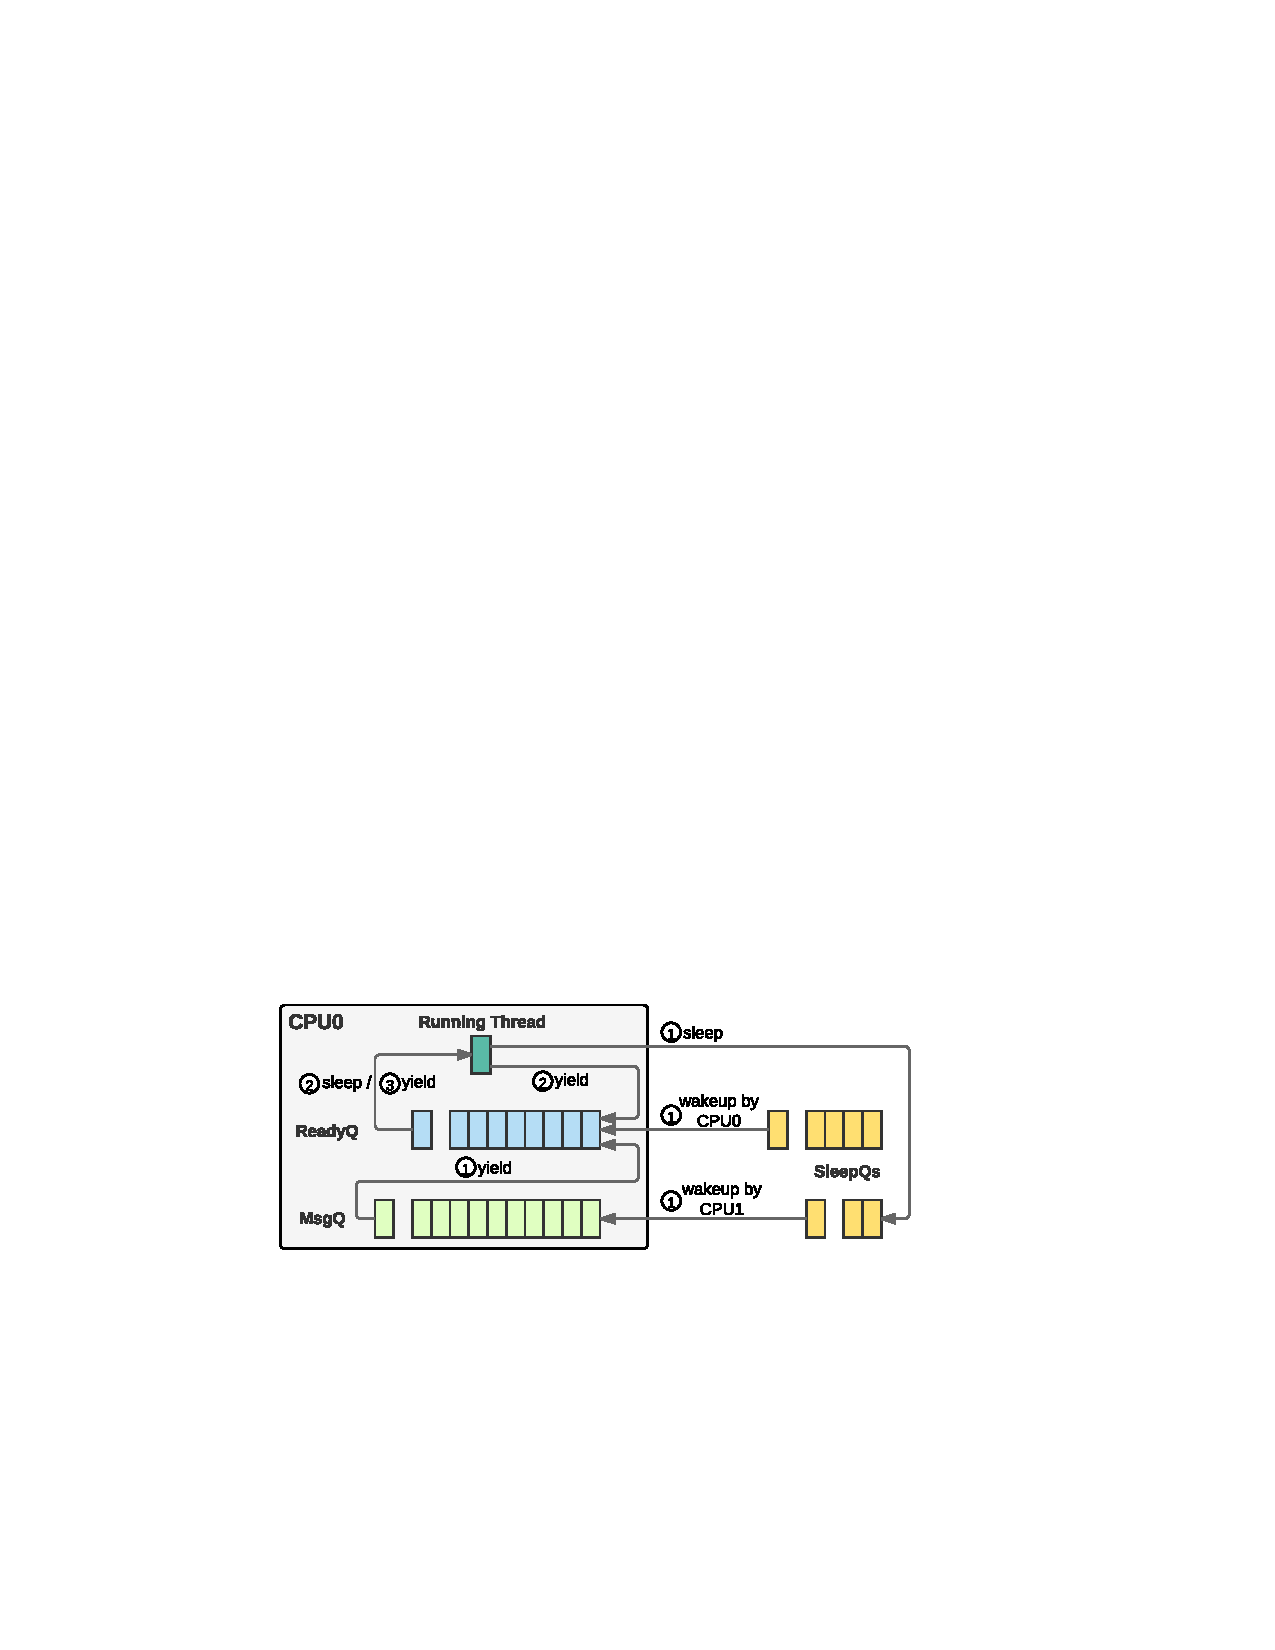
\includegraphics[scale=.72]{figs/scheduler} 
\end{center}
\vspace{-10pt}
\caption{Scheduling procedures of \texttt{yield}, \texttt{sleep},
and \texttt{wakeup}.}
\label{fig:exp:fig:scheduler}
\vspace{-10pt}
\end{figure}

\begin{figure}
\lstinputlisting [language = C, multicols=2] {source_code/thread_management.c}
\caption{Implementation of the Scheduler Module}
\label{fig:exp:scheduler}
\end{figure}

\vspace{-3pt}
\paragraph{Thread-local machine model}
can be introduced based on the thread management.
The first step is to 
extend the environment context
with a \emph{software scheduler} (\ie, abstracting the concrete
scheduling procedure), resulting in a new environment context $\oracle_{ss}$.
The scheduling primitives 
generate the $\event{yield}$ and
$\event{sleep}$
events, and $\oracle_{ss}$ responds with the next
thread ID to execute.
One invariant we have to require on $\oracle_{ss}$
is that a sleeping thread can be rescheduled only after 
a $\event{wakeup}$ event is generated.
The second step is to introduce
the \emph{active thread set}
to represent the target threads on the \emph{active CPU},
and extend the $\oracle_{ss}$
with the \emph{context threads},
\ie, the rest of the threads running on 
the active CPU. The composition structure is similar to the one of Lemma~\ref{lemma:compose}.
In this way,
higher layers can be built upon a thread-local machine model
with a single active thread on the active CPU
(\cf Fig.~\ref{fig:spec:refine_layer}).

\vspace{-3pt}
\paragraph{Starvation-free condition variable}
A \emph{condition variable} is a synchronization object
that enables a thread to efficiently wait for a change to be made 
to a shared state (protected by a lock). 
To make sure there is no starvation inside the \mCTOS\ kernel,
every thread waiting on a condition variable (CV) needs to be signaled within 
a certain bounded number of execution steps.
We have implemented a starvation-free version of condition variable
using a FIFO blocking bounded queue (FIFOBBQ) of condition variables,
following a similar idea to that presented in \cite[fig~5.14]{ospp11}.
However, we have found a bug in the implementation shown in that textbook \cite{anderson16}.
In some cases, the system can get stuck by allowing all the signaling and
waiting threads to be asleep simultaneously, or the system can arrive at
a dead end where the threads on the remove queue (rmvQ) can no longer be woken up.
In {\CTOS}, this issue is fixed by postponing the removal of
the CV of a waiting thread from the queue, until the waiting thread finishes its
work. As shown in Fig.~\ref{fig:exp:fifo}, the remover is now responsible
for removing itself from the rmvQ (line 23) and waking up the next element
in the rmvQ (line 26).

\begin{figure}
\lstinputlisting [language = C, multicols=2] {source_code/fifoq.c}
\vspace{-5pt}
\caption{Implementation of remove method of FIFOBBQ.}
\label{fig:exp:fifo}
\vspace{-10pt}
\end{figure}

\paragraph{IPC}
We have implemented and verified a single-copy
inter-process communication (IPC) protocol using condition variables
and the FIFO Blocking Bounded Queue.
Additionally, we have verified a
zero-copy IPC for user programs that is built on top of the
shared memory infrastructure.
\ignore{
\begin{figure}
\lstinputlisting [language = C, multicols=2] {source_code/ipc.c}
\caption{Implementation of Single-Copy IPC}
\label{fig:exp:ipc}
\end{figure}

\vspace{-3pt}
\paragraph{Trap handler}
\label{sec:base:trapm}

\ignore{
\begin{figure}
\begin{center}
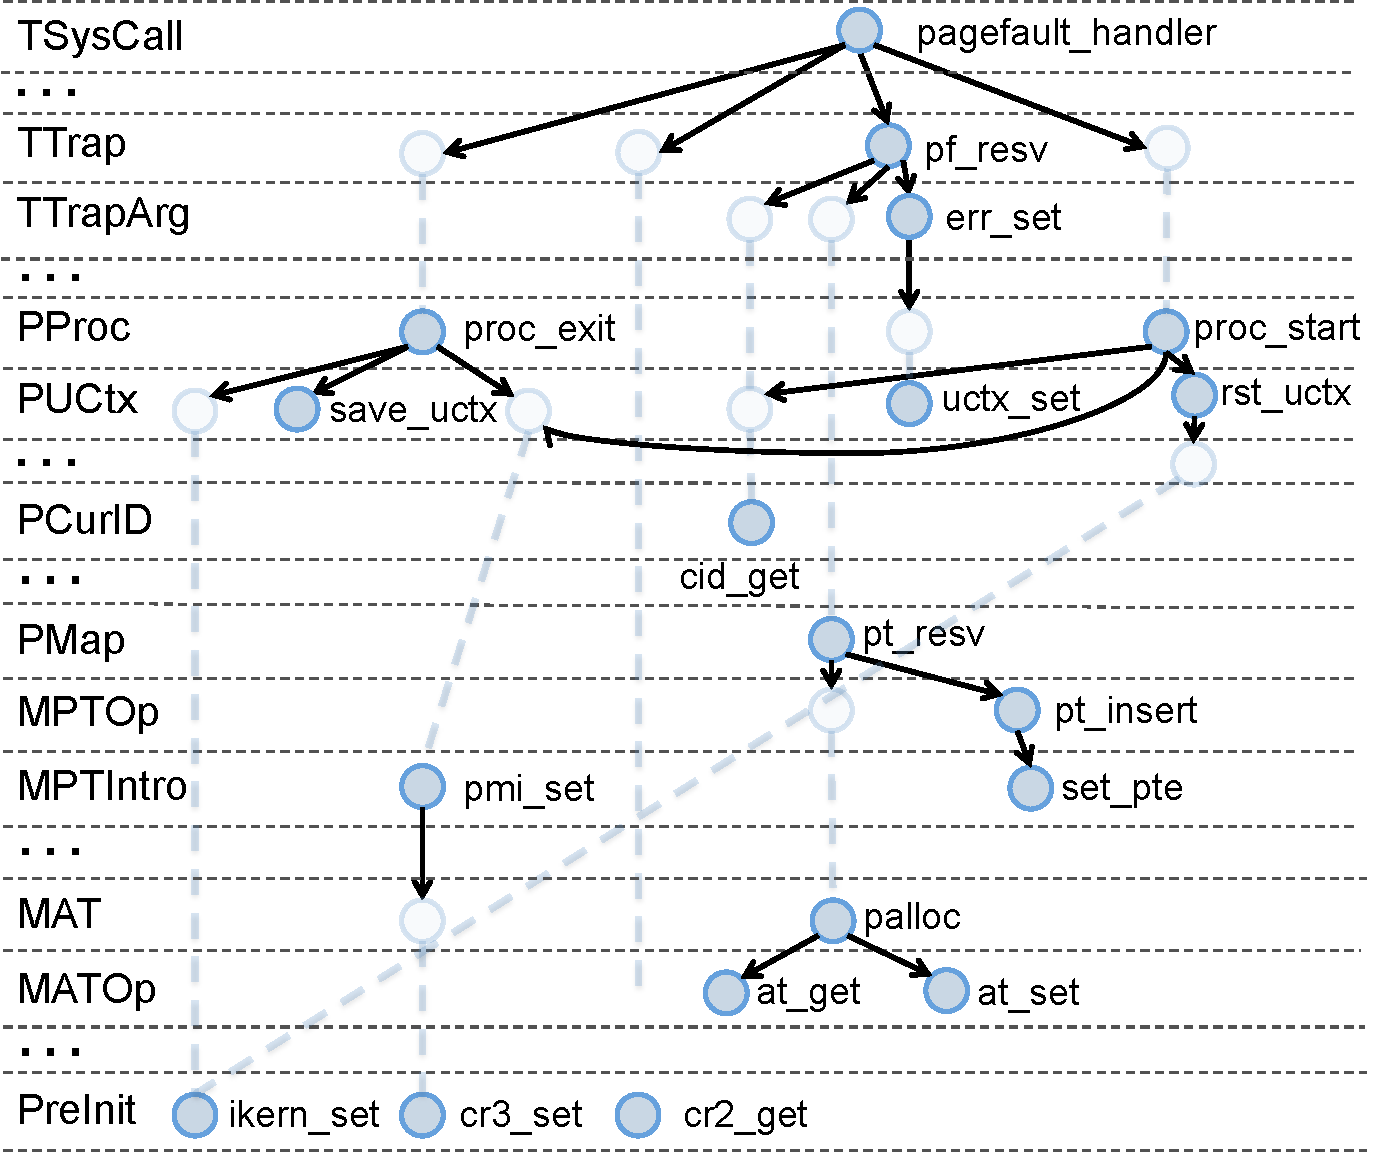
\includegraphics[scale=0.33]{figs/pagefault2}	
\caption{Call graph of page fault handler}
\label{fig:base:pagefault}
\end{center}
\vspace*{-14pt}
\end{figure}
}
specifies the behaviors of exception handlers
(\eg, page fault handler), interrupt handlers (\eg, serial port),
and system calls (\eg. IPC). It also specifies the behavior of ring switch and saving/restoring trap frames.
}
\ignore{
For example, a page fault at the user level traps into the kernel, saves the
current trap frame (done by both the hardware and software), and then jumps
to the page fault handler.
The page fault handler reserves a page for \texttt{PFLA} (if necessary)
and returns to the user level by restoring the saved user context.
The verification of the page fault handler depends on objects
introduced at various abstraction levels. 
\ronghui{So what? Everybody knows what is a page fault?}
% (see Fig.~\ref{fig:base:pagefault}).
}

\ignore{
Therefore, the behavior of the page fault handler is interpreted by
the concrete first-class code pointer until all the dependent layer
objects are introduced.  Then the handler code is verified and
the behavior is interpreted using its abstract atomic specification.
}


To further simplify the reasoning about user code, we have implemented and
verified the user level system call libraries directly in the user space.
Since our machine semantics models hardware behaviors
like paging and ring switch, the specifications of user system call
libraries closely corresponds to the real execution model in the actual
hardware. With this \emph{atomic} system call semantics in the user level,
the user code can be proved much more easily.

The top layer of \mCTOSbase{} offers a set of system calls for user programs, 
such as IPC calls and calls to trigger the scheduler.
The specifications of system calls are defined and verified at the user level
by wrapping the system call handler's specification
with the ring switch specification.
We can reason about user-level programs directly with these atomic system calls' specifications.


\ignore{
\newman{Already in Section 2}
\subsection{Other properties}
Except for the above features, we also prove the following properties of \mCTOSbase{}:
\begin{itemize}
\item Since the contextual refinement is termination sensitive, we prove the total
correctness of our kernel, meaning that our kernel will not get stuck
and all system calls for user program will terminate.
\item There is no integer overflow inside the kernel.
\item There is not stack overflow inside the kernel. (Statically checked by the analysis tool,
refer to Quentin's work)
\item All the pointers stored in the kernel objects are valid.
\end{itemize}
}
